\documentclass[10pt]{article}

\usepackage{graphicx}
\usepackage{amsmath,amsfonts,amssymb}

\usepackage{hyperref}  % for urls and hyperlinks


\setlength{\textwidth}{6.2in}
\setlength{\oddsidemargin}{0.3in}
\setlength{\evensidemargin}{0in}
\setlength{\textheight}{8.9in}
\setlength{\voffset}{-1in}
\setlength{\headsep}{26pt}
\setlength{\parindent}{0pt}
\setlength{\parskip}{5pt}




% a few handy macros

\newcommand\matlab{{\sc matlab}}
\newcommand{\goto}{\rightarrow}
\newcommand{\bigo}{{\mathcal O}}
\newcommand{\half}{\frac{1}{2}}
%\newcommand\implies{\quad\Longrightarrow\quad}
\newcommand\reals{{{\rm l} \kern -.15em {\rm R} }}
\newcommand\complex{{\raisebox{.043ex}{\rule{0.07em}{1.56ex}} \hskip -.35em {\rm C}}}


% macros for matrices/vectors:

% matrix environment for vectors or matrices where elements are centered
\newenvironment{mat}{\left[\begin{array}{ccccccccccccccc}}{\end{array}\right]}
\newcommand\bcm{\begin{mat}}
\newcommand\ecm{\end{mat}}

% matrix environment for vectors or matrices where elements are right justifvied
\newenvironment{rmat}{\left[\begin{array}{rrrrrrrrrrrrr}}{\end{array}\right]}
\newcommand\brm{\begin{rmat}}
\newcommand\erm{\end{rmat}}

% for left brace and a set of choices
\newenvironment{choices}{\left\{ \begin{array}{ll}}{\end{array}\right.}
\newcommand\when{&\text{if~}}
\newcommand\otherwise{&\text{otherwise}}
% sample usage:
%  \delta_{ij} = \begin{choices} 1 \when i=j, \\ 0 \otherwise \end{choices}


% for labeling and referencing equations:
\newcommand{\eql}{\begin{equation}\label}
\newcommand{\eqn}[1]{(\ref{#1})}
% can then do
%  \eql{eqnlabel}
%  ...
%  \end{equation}
% and refer to it as equation \eqn{eqnlabel}.  


% some useful macros for finite difference methods:
\newcommand\unp{U^{n+1}}
\newcommand\unm{U^{n-1}}

% for chemical reactions:
\newcommand{\react}[1]{\stackrel{K_{#1}}{\rightarrow}}
\newcommand{\reactb}[2]{\stackrel{K_{#1}}{~\stackrel{\rightleftharpoons}
   {\scriptstyle K_{#2}}}~}

% Parts:

% set enumerate to give parts a, b, c, ...  rather than numbers 1, 2, 3...
\renewcommand{\theenumi}{\alph{enumi}}
\renewcommand{\labelenumi}{(\theenumi)}

% set second level enumerate to give parts i, ii, iii, iv, etc.
\renewcommand{\theenumii}{\roman{enumii}}
\renewcommand{\labelenumii}{(\theenumii)}

  % input some useful macros

\begin{document}

% header:
\hfill\vbox{\hbox{AMath 585}
\hbox{Homework \#6}\hbox{Due Thursday, March 12, 2020}}

\vskip 5pt

Homework is due to Canvas by 11:00pm PDT on the due date.

To submit, see
\url{https://canvas.uw.edu/courses/1352870/assignments/5284853}



%--------------------------------------------------------------------------
\vskip 1cm
\hrule
{\bf Problem 1.}
Consider the BVP $u''(x) = 0$ on $0\leq x \leq 1$ with Dirichlet boundary
conditions $u(0)=0$ and $u(1)=1$.  The exact solution is $u(x)=x$.

Discretize with the standard centered approximation using $m$ equally spaced
interior points.  If we apply the Conjugate-Gradient method with initial
data $u_i^{[0]} = 0$ for $i=1,~2,~\ldots,~m$ then we see the sort of behavior
that is illustrated in the plots below for the case $m=4$.  For $k<m$ 
the approximate 
solution is always piecewise linear and has $u_i^{[k]} = 0$ for $i \leq m-k$.
After $m$ iterations, $u^{[m]}$ is equal to the exact solution.

\hfil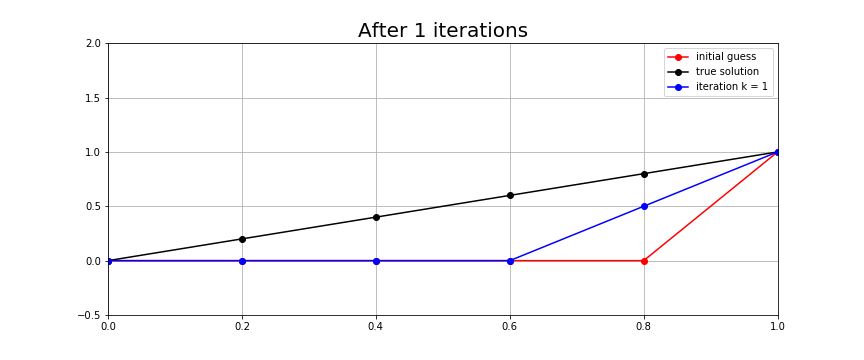
\includegraphics[width=4.5in]{frame1.png}\hfil

\hfil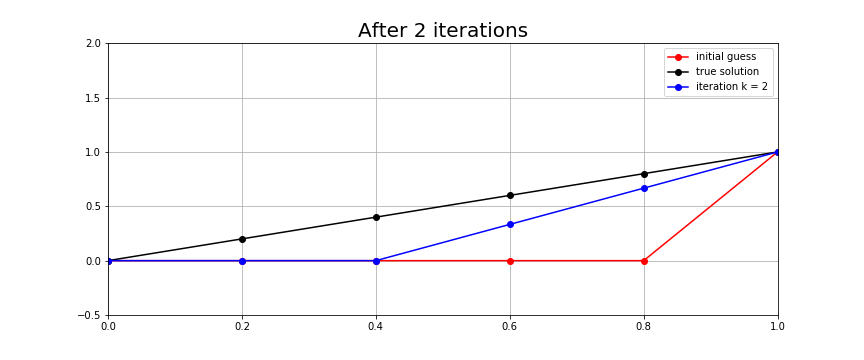
\includegraphics[width=4.5in]{frame2.png}\hfil

\hfil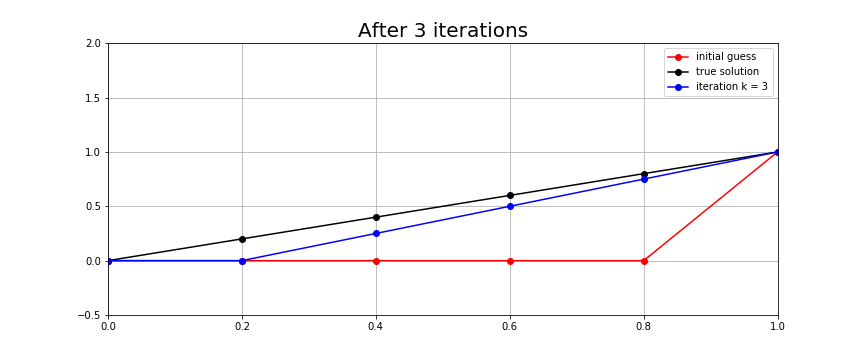
\includegraphics[width=4.5in]{frame3.png}\hfil

\newpage
(a) For the case $m=3$, work through the C-G algorithm by hand to explicitly
calculate the vectors $r^{[k]},~b^{[k]},$ and $u^{[k]} \in \reals^3$ in
each iteration.  This should help you see why the behavior seen in
the plots makes sense.

(b) To show this behavior is seen for general $m$, show by induction that each
residual $r^{[k]}$ is a unit vector (all zeros except in one element). 
Hint: Use the fact that we know that all the residuals generated in C-G
are pairwise orthogonal to one another, and that the only elements that can
change from one iteration to the next are those in which the search direction
$b^{[k]}$ has nonzero components, which can also be determined in general.

(c) Explain how the result of (b) implies the behavior seen in the plots.

% uncomment the next two lines if you want to insert solution...
%\vskip 1cm
%{\bf Solution:}

% insert your solution here!

%--------------------------------------------------------------------------
\vskip 1cm
\hrule
{\bf Problem 2.}
Consider a linear system $Au=f$ in which the matrix $A$ is {\bf not} symmetric
positive definite, so C-G cannot be applied directly.

(a) Show that if $A$ is nonsingular then the matrix $B = A^TA$ is symmetric
positive definite.

(b) So one approach to solving $Au = f$ is multiply both sides by $A^T$ to get
$Bu = A^Tf$ and then solve this system with C-G.  The problem with this approach 
is that the condition number increases.  Show that the 2-norm condition
number of $B$ is the square of the 2-norm condition number of $A$.

(c) On page 93 it is noted that applying C-G to the two-dimensional Poisson
problem $Au = f$ on an $m$ by $m$ grid (with second order centered differencing) 
requires $O(m^3)$ work to converge to a fixed
tolerance.  Suppose we multiplied both sides by $A^T$ as described above (even 
though not necessary here since $A$ is already SPD) and solved the resulting
system (which is still SPD) by C-G.  What order of work would now be required
to reach a fixed tolerance?  

(d) Given that the global error for this discretization is $O(h^2) = O(1/m^2)$
for smooth solutions, it makes more sense to look at the work required to
get the error in the C-G solution down to this level.  How does this change
the work estimates given above, both for solving $Au=f$ and $A^TAu = A^Tf$? 

\vskip 5pt
{\em Note:} there are better approaches for nonsymmetric matrices than the 
approach described above that do not magnify the condition number, 
see Section 4.4 and other references.


% uncomment the next two lines if you want to insert solution...
%\vskip 1cm
%{\bf Solution:}

% insert your solution here!


%--------------------------------------------------------------------------
\vskip 1cm
\hrule
{\bf Problem 3.}
As in the previous homework, consider the one-dimensional BVP 
\[
\frac{d}{dx}\left(\kappa(x) u'(x)\right) = 0
\]
on $0 \leq x  \leq 1$ with Dirichlet boundary conditions $u(0)=0$ and $u(1)=1$, 
again discretizing this problem using the system (2.71) in the text.  (Or
negate it if you prefer, to make it positive definite.)

Consider the piecewise constant diffusivity
\[
\kappa(x) = \begin{cases}
\epsilon & \text{if~} x < 0.5,\\
1 & \text{if~} x > 0.5.
\end{cases}
\]
where $\epsilon > 0$.

(a)  Generalizing what you did in HW5, determine the exact solution, 
in terms of the parameter $\epsilon$.

(c) Implement the conjugate gradient method for this problem. 
For the convergence test require  $\|r^{[k]}\|_2 < 10^{-14}$.
Allow more than $m$ iterations, if necessary.

Make semilogy plots of the max-norm
of the error and the 2-norm of the residual as a function of iteration $k$
for the case $m=19$ with $\epsilon = 0.1$.  Also try $\epsilon = 10^{-3}$.
You should observe that more than $m$ iterations are required to get good
results.  Comment on the behavior of the iterates in each case.

(d) Implement the preconditioned C-G algorithm (PCG) using the 
diagonal preconditioner and observe that this greatly 
improves the convergence behavior.  

{\em Note:} Make sure you do this in a way for which $M$ is symmetric
positive definite and not negative definite, as discussed in the notebook
{\tt PCG.ipynb} and video that goes with it.  This also contains corrections to 
some typos in the PCG algorithm written on page 95.

The notebook {\tt DarcyFlow.ipynb} provides an implementation of the 
PCG algorithm for the two dimensional version of this problem that 
may be useful to follow.


% uncomment the next two lines if you want to insert solution...
%\vskip 1cm
%{\bf Solution:}

% insert your solution here!


%--------------------------------------------------------------------------
\vskip 1cm
\hrule
{\bf Problem 4.}
Consider the same problem as in Problem 3 but now on the interval 
$0\leq x \leq 4$ with Dirichlet boundary conditions and with $m=3$ internal
grid points (so $h=1$ for convenience).  Now put the jump in $\kappa$ at the
midpoint $x=2$:
\[
\kappa(x) = \begin{cases}
\epsilon & \text{if~} x <2,\\
1 & \text{if~} x > 2.
\end{cases}
\]

(a) Write out the $3\times 3$ matrix $A$ explicitly in this case.

(b) Write out the matrix $M$ that would be used as the "diagonal
preconditioner" in this case.  Also compute $B = M^{-1}A$ and observe
that it is not symmetric.

(c) In this case we can choose $C$ to be diag$(\sqrt{M_{ii}})$. Write out the
matrix $\tilde A = C^{-T}AC^{-1}$ in this $3\times 3$ case and observe that
it is symmetric.

(d) For the case $\epsilon = 10^{-4}$ compute the eigenvalues and
2-norm condition number of $A$ and $B$ (recall that those of $\tilde
A$ agree with those of $B$, but $B$ is easier to work with).  You
can use the {\tt eig} function in Numpy or Matlab, or do it by hand.

(e)  Note that as $\epsilon \goto 0$ the matrix $A$ approaches a
singluar matrix and the condition number blows up.  What does the
condition number of $B$ approach as $\epsilon \goto 0$?
(You should be able to compute this analytically by looking at the
limiting matrix.)

% uncomment the next two lines if you want to insert solution...
%\vskip 1cm
%{\bf Solution:}

% insert your solution here!

%--------------------------------------------------------------------------

\end{document}
